\documentclass{article}
\usepackage[polish]{babel}
\usepackage{amssymb}
\usepackage{graphicx}
\title{Sprawozdanie z Laboratorium 1}
\author{
  Hubert Rotkiewicz 193421 \and 
  Paweł Dolak 193582
}
\begin{document}
\maketitle
\begin{figure}[h]
  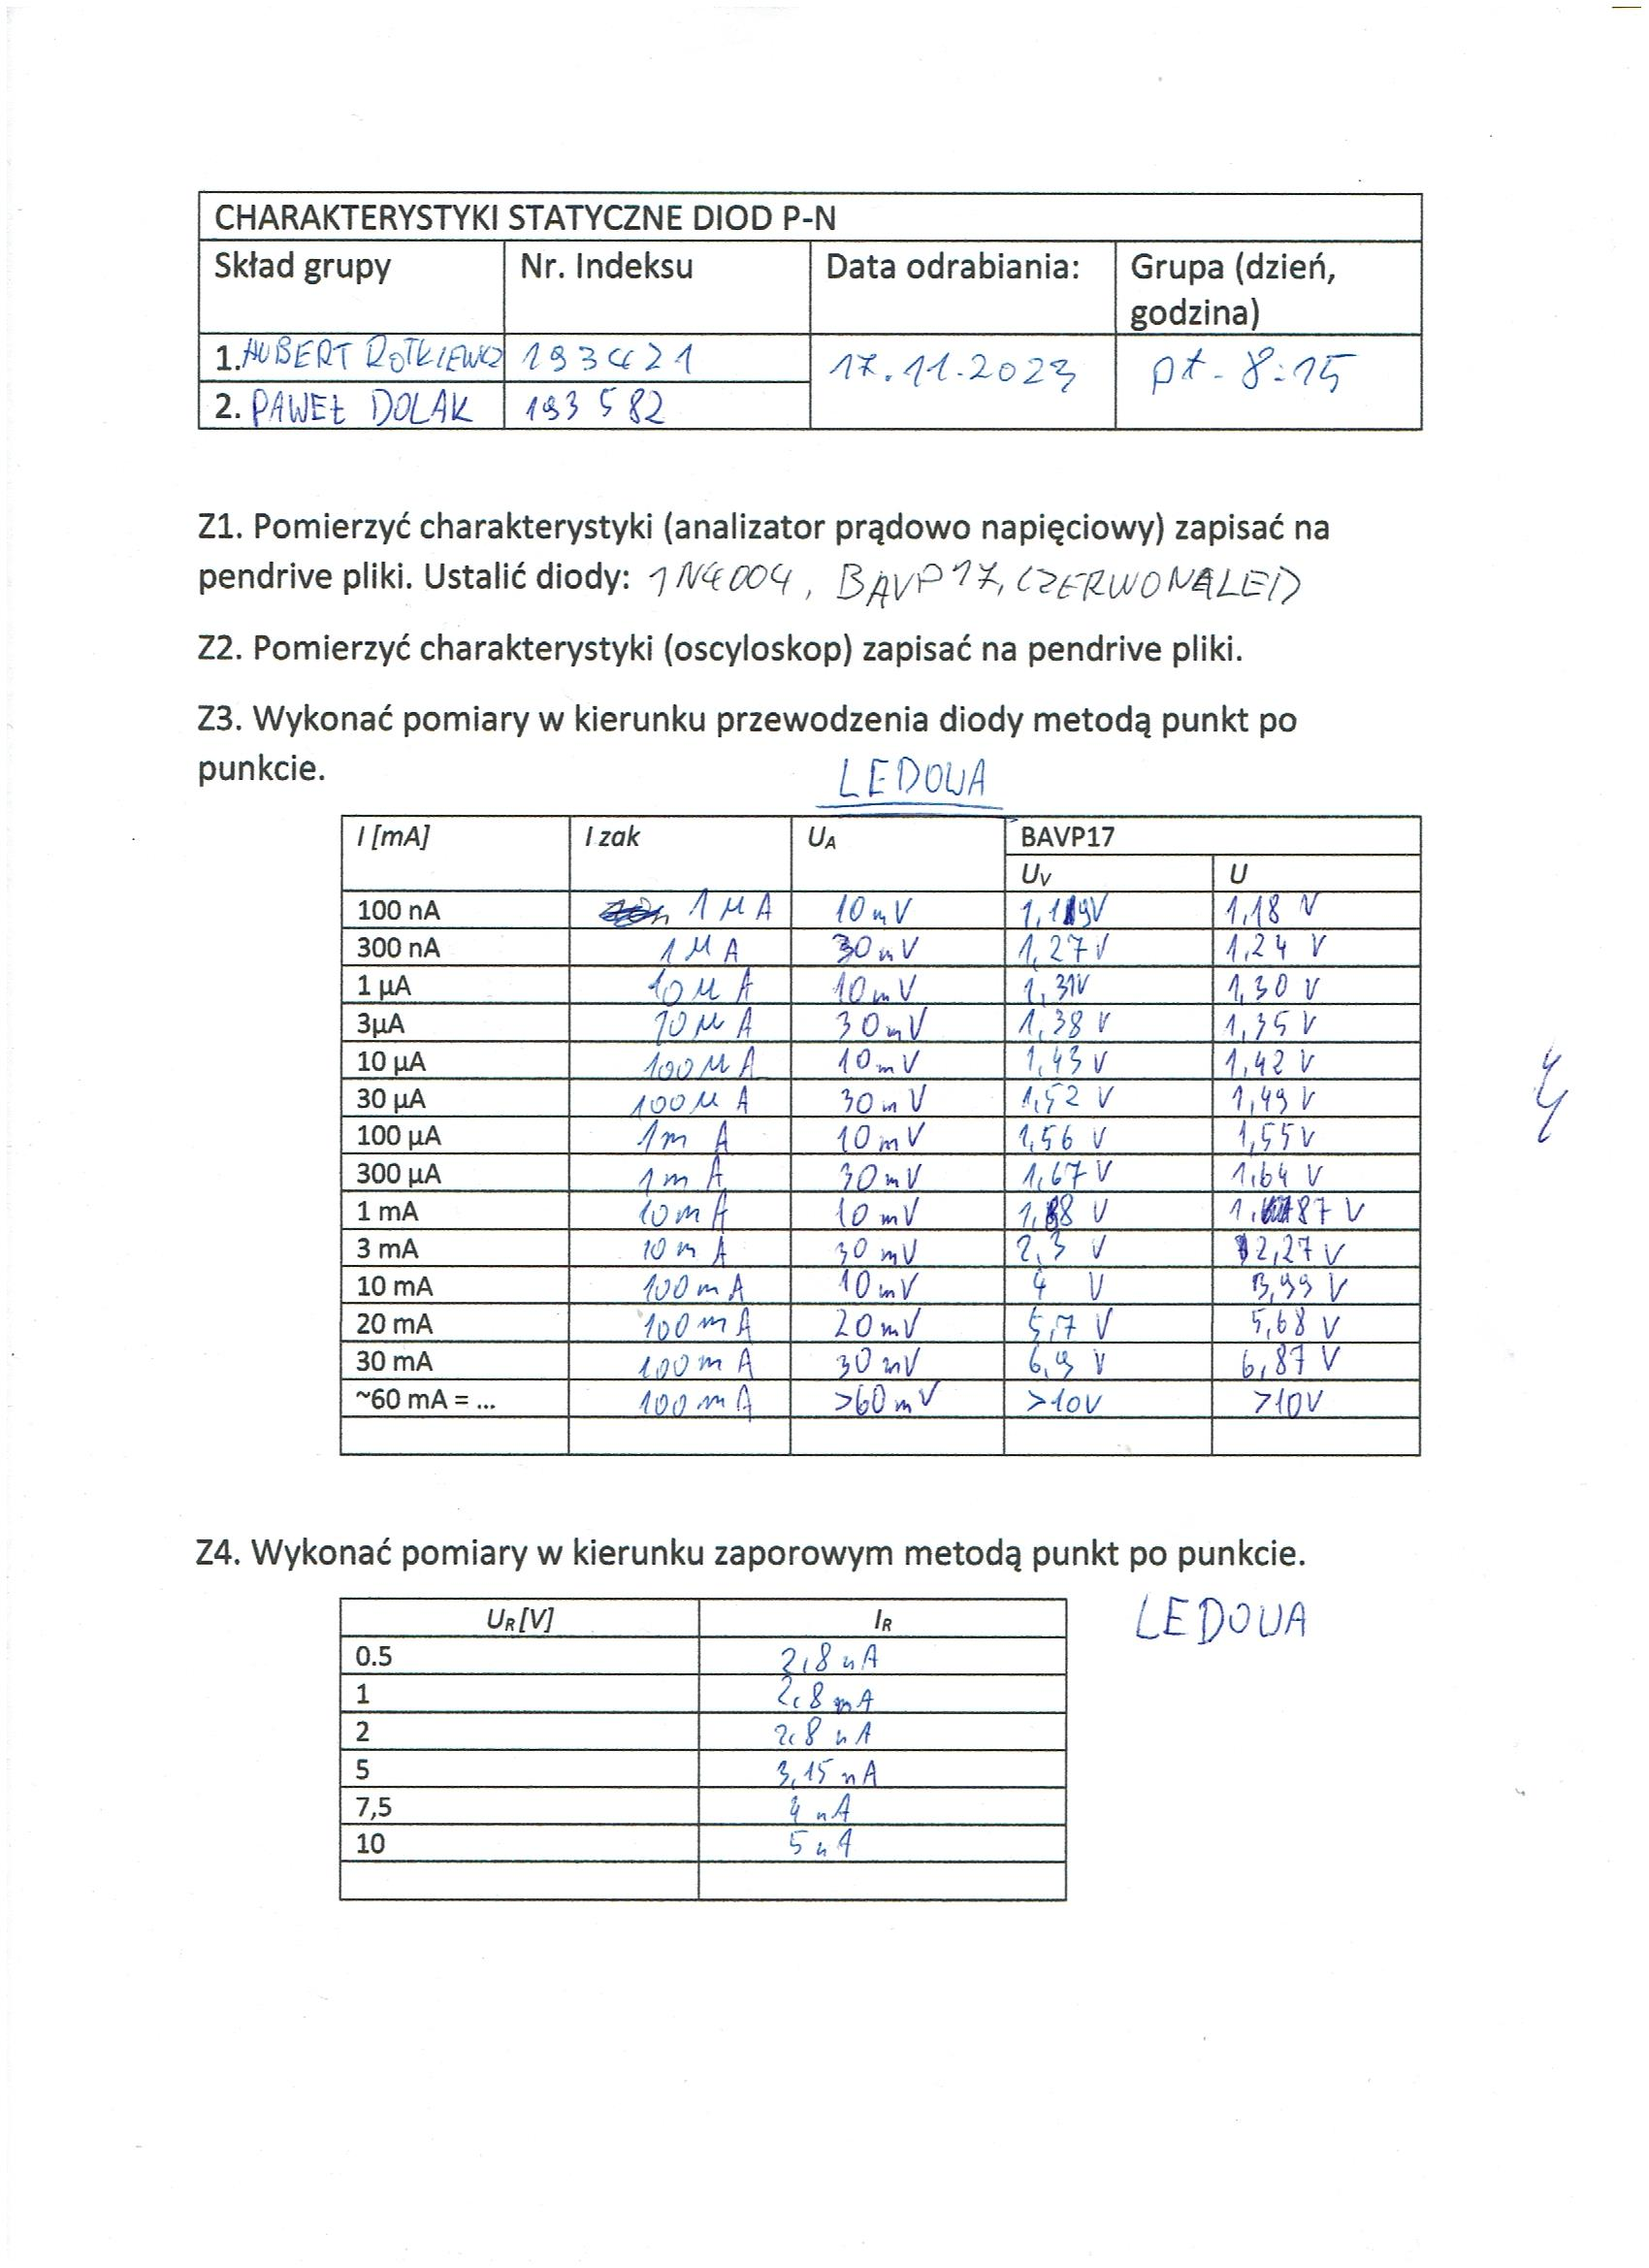
\includegraphics[scale=0.6]{./img/Protokol_pp_cw1.jpg}
\end{figure}
\clearpage
\raggedright
\section{Wzory używane do obliczeń}

Korzystając ze wzoru można policzyć prąd nasycenia diody\[
  I = I_s \cdot e^{\frac{U}{nV_t}} \Rightarrow
  I_s = \frac{I}{e^{\frac{U}{nV_t}}} 
\]
Obliczenia dla poszczególnych diod: \\
Współczynnik nieidealności - n można wyznaczyć z następującego wzoru \[
  n = \frac{\Delta{U}}{V_t \Delta{\ln(I)}}
\]
Obliczenia dla poszczególnych diod: \\
Współczynnik $r_s=\frac{U`}{\Gamma}$ - rezystancji szeregowej, został wyznaczony dla jak największej wartości zmierzonego prądu diody. Odczytując z wykresu otrzymano następujący wynik:\\
Obliczenia dla poszczególnych diod: \\
Oznaczenia we wzorach:
\raggedright
\\ U - napięcie na diodzie\\ n - współczynnik nieidealności\\ $V_t$ - napięcie termiczne, założono wartość 26mV\\ 
$I_s$ - prąd nasycenia diody\\ I - prąd płynący przez diodę\\ $r_s$ - rezystancja szeregowa\\ $\Gamma$ - największa wartość zmierzonego prądu diody \\
U` - różnica pomiędzy wartością napiecia obserwowaną na diodze, a napięciem, które panowałoby na tej diodzie, gdyby $r_s$ było równe 0\\
\clearpage
\raggedright
\section{Zadanie 1}
\subsection{a)}
\centering
Dostaliśmy polecenie od prowadzącej laboratoria, aby nie wykonywać zadania Z1. Więc nie posiadamy potrzebnych danych do wykonania tego zadania.
\raggedright
\subsection{b)} 
\centering
\begin{figure}[h]
  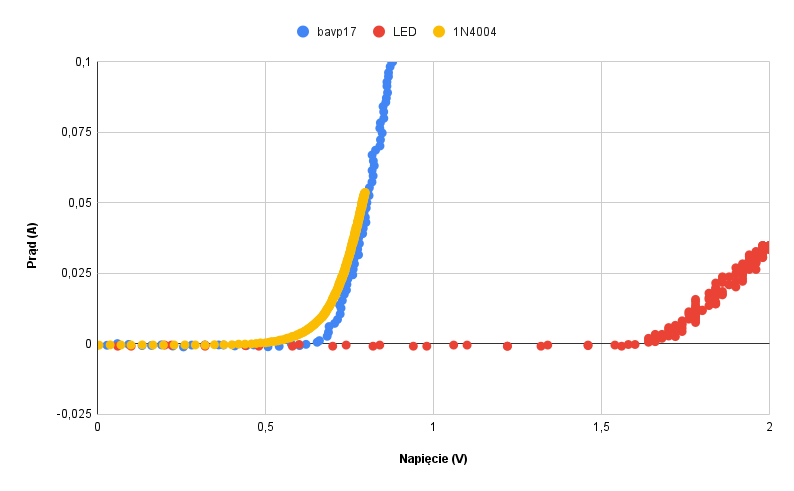
\includegraphics[scale=0.5]{./img/chart.png}
  \caption{Charakterystyki prądowo-napięciowe badanych diod}
\end{figure}
Jak widać na załączonym wykresie, Dioda czerwona LED ma największe napięcie progowe wynoszące około $U \approx 1.65$. Diody BAVP17 i 1N4004 mają zbliżone do siebie charakterystyki, 
jednakże dioda 1N4004 ma mniejsze napięcie progowe. 
\raggedright
\subsection{c)}
\centering
Rożnice wartości spadków napięć jak i w prądzie przewodzenia wynikają w głównej mierze z rożnicy w budowie diody tzn. diody krzemowe są wykonane z  pierwiastków o innych wartościach przewodzenia niż pierwiastki z któych zbudowana jest dioda LED. Dodatkowo istotna jest również przerwa energetyczna, którą dioda LED posiada większą. Miedzy diodami krzemowymi nie ma aż tak znaczących różnic i wynikają one głownie z ich specyfikacji.
\raggedright
\section{Zadanie 2}
% \begin{figure}[h!]
%   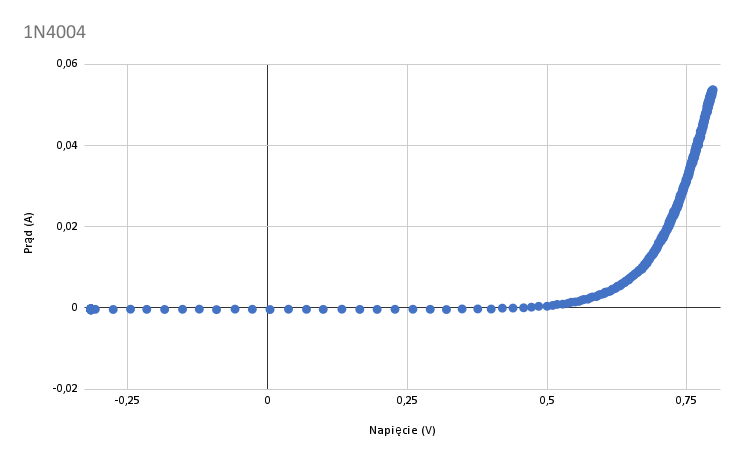
\includegraphics[scale=0.3]{./img/1N4004.png}
%   \caption{Charakterystyka prądowo-napięciowa diody 1N4004}
%   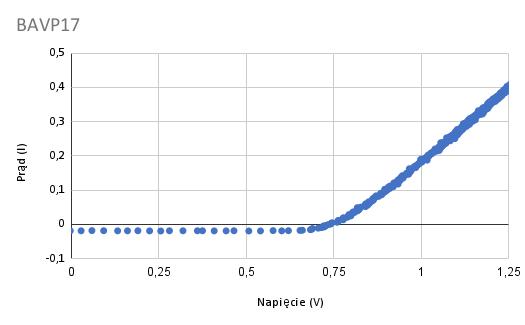
\includegraphics[scale=0.4]{./img/BAVP17.png}
%   \caption{Charakterystyka prądowo-napięciowa diody BAVP17}
%   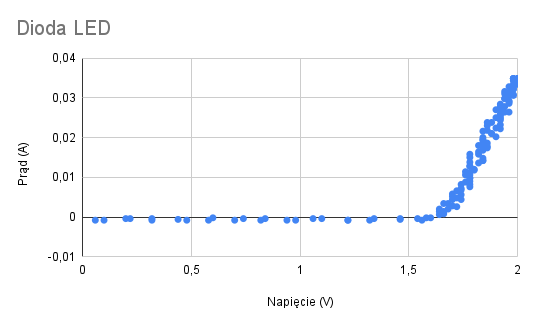
\includegraphics[scale=0.4]{./img/LED.png}
%   \caption{Charakterystyka prądowo-napięciowa diody czerwonej LED}
% \end{figure}
Dostaliśmy polecenie od prowadzącej laboratoria, aby nie wykonywać zadania Z1. Więc nie posiadamy potrzebnych danych do wykonania tego zadania.
\raggedright
\section{Zadanie 3}
\centering
\begin{figure}[h]
  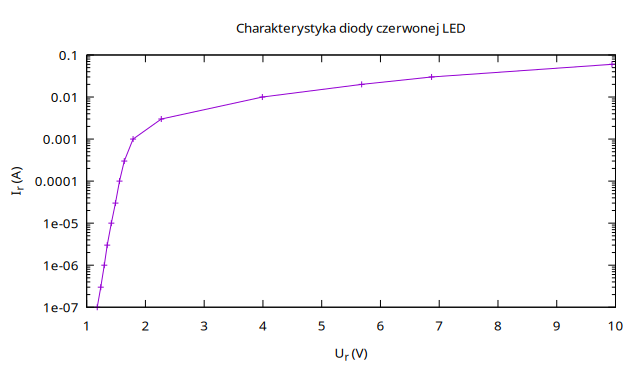
\includegraphics[scale=0.5]{./img/Z3_U.png}
  \caption{Wykres prądu w funkcji napięcia dla diody czerwonej LED. Przedstawiony w skali logarytmiczno-liniowej}
\end{figure}
Korzystając z wcześniej przedstawionych wzorów i wartości odczytanych z wykresu lub tabeli, można wyznaczyć parametry diody: \\
Rezystancja szeregowa, obliczona dla $\Gamma=60mA$, czyli największego zmierzonego prądu płynącego przez diodę.  $r_s=\frac{U'}{\Gamma} = \frac{10-9.94}{60 \cdot 10^{-3}}=1$
współczynnik nieidealności diody: \[n = \frac{1.49-1.42}
{26 \cdot 10^{-3} \cdot (\ln{(30 \cdot 10^{-6})}-\ln{(10 \cdot 10^{-6}}))} \approx 2.45\]
Prąd nasycenia diody, obliczony dla punktu $(1.64,300\cdot10^{-6})$: \[I_s=\frac{300 \cdot 10^{-6}}{e^{\frac{1.64}{2.45 \cdot 26 \cdot 10^{-3}}}} \approx 1.97657... \cdot 10^{-15}\]

\clearpage
\raggedright
\section{Zadanie 4}
\begin{figure}[h!]
\centering
  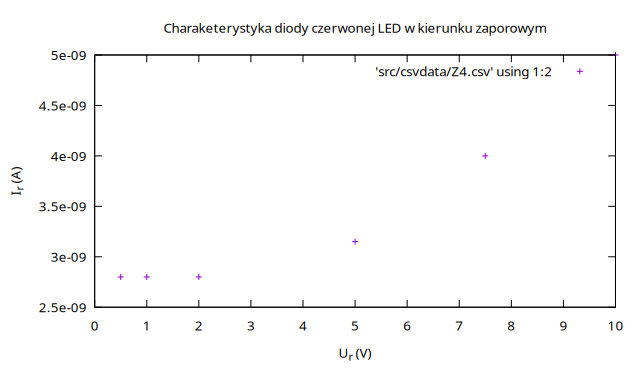
\includegraphics[scale=0.5]{./img/Z4.png}
  \caption{Wykres prądu w funkcji napięcia dla diody czerwonej LED. Przedstawiony w skali logarytmiczno-liniowej}
\end{figure}
\centering
Z danych wynika, że dla $U_r = -5$ prąd płynący przez diodę wynosi $I_r=3.15nA$.
W złączu idealnym, przy polaryzacji zaporowej $ J \approx J_s \cdot [\exp{(\frac{qV}{k_BT})}-1] \rightarrow 
I \approx -I_s$ w zmierzonym przypadku prąd $I_s=1.97fA$, a więc jest on znacznie mniejszy niż $I_r$. 
Prąd na diodzie był mierzony używając miernika U726 firmy Meratronik. Mierniki te były produkowane w 1976 roku,
więc można przypuszczać, że ich dokładność jest wątpliwa. Jedyną note katalogową jaką udało się znaleźć była
napisana w języku niemieckim, a więc niezrozumiała dla autorów tego sprawozdania.
Jednakże obydwa prądy są bardzo małe, w zwykłej analizie obwodu można je pominąć. 








